%%%%%%%%%%%%%%%%%%%%%%% file typeinst.tex %%%%%%%%%%%%%%%%%%%%%%%%%%%%%%
%
% This is the LaTeX source for the instructions to authors using
% the LaTeX document class SVMultln with class option 'lnicst'
% for contributions to the Lecture Notes of the Institute for
% Computer Sciences, Social-Informatics and
% Telecommunications Engineering series.
% www.springer.com/series/XXXX       Springer Heidelberg 2007/08/05
%
% It may be used as a template for your own input - copy it
% to a new file with a new name and use it as the basis for
% your article. It contains a few tweaked sections to demonstrate
% features of the package, though.
%
% If you have not much experiences with Springer LaTeX support,
% you should better use the special demonstration file "lnicst.tex"
% included in the LaTeX package for LNICST as template.
%
%%%%%%%%%%%%%%%%%%%%%%%%%%%%%%%%%%%%%%%%%%%%%%%%%%%%%%%%%%%%%%%%%%%%%%%%

%\documentclass[lnicst,sechang,a4paper]{svmultln}
%\documentclass[12pt]{llncs}
\documentclass[runningheads,a4paper]{llncs} %this is for NSS


\usepackage{amssymb}
\setcounter{tocdepth}{3}
\usepackage{graphicx}


%\usepackage{amssymb}
%\setcounter{tocdepth}{3}
%\usepackage{graphicx}
%\usepackage{fancyhdr}
%\usepackage{lastpage}

\usepackage{url}

%\urldef{\mailsa}\path|{alfred.hofmann, ursula.barth, ingrid.haas, frank.holzwarth,|
%\urldef{\mailsb}\path|anna.kramer, leonie.kunz, christine.reiss, nicole.sator,|
%\urldef{\mailsc}\path|erika.siebert-cole, peter.strasser, lncs}@springer.com|    
%\newcommand{\keywords}[1]{\par\addvspace\baselineskip
%\noindent\keywordname\enspace\ignorespaces#1}


%added by the author himself
\usepackage{color}
\usepackage[numbers]{natbib}
\usepackage{calc}
\usepackage{siunitx}
\DeclareSIUnit\mt{\milli\tesla} %% A method for say short cut or new unit!
\sisetup{inter-unit-product = {-}}

%added by kimmo
%\setlength\parskip{12pt}
%\setlength\parindent{0pt}
%\pagestyle{fancy}
%\fancyhf{} 
%\fancyfoot[C]{\thepage\ / \pageref{LastPage}}
%\renewcommand{\headrulewidth}{0pt}

\begin{document}

\mainmatter  % start of an individual contribution

% first the title is needed
\title{Concealing IMSI in 5G Network Using Identity Based Encryption}
%Concealing IMSI in 5G Network Using Identity Based Cryptography

% a short form should be given in case it is too long for the running head
\titlerunning{Concealing IMSI Using Identity Based Encryption} 

% the name(s) of the author(s) follow(s) next
%
% NB: Chinese authors should write their first names(s) in front of
% their surnames. This ensures that the names appear correctly inlso
% the running heads and the author index.
%
\author{Mohsin Khan%
%%\thanks{Please note that the LNICST Editorial assumes that all authors have used
%%the western naming convention, with given names preceding surnames. This determines
%%the structure of the names in the running heads and the author index.}%
\and Valtteri Niemi\\
\email{mohsin.khan@helsinki.fi, valtteri.niemi@helsinki.fi}
}  %

\authorrunning{Mohsin Khan \and Valtteri Niemi}
% (feature abused for this document to repeat the title also on left hand pages)

% the affiliations are given next
\institute{University of Helsinki, Department of Computer Science,\\
P.O. Box 68 (Gustaf H\"allstr\"omin katu 2b)\\
FI-00014 University of Helsinki\\
Finland\\
\url{https://www.cs.helsinki.fi/en}
}

%relationship stu
%
% NB: a more complex sample for affiliations and the mapping to the
% corresponding authors can be found in the file "lnicst.dem",
% that is contained in the LNICST LaTeX support package.
%

%%%\toctitle{Lecture Notes in Computer Science}
%%%\tocauthor{Authors' Instructions}
\maketitle


\begin{abstract}
The aspirations for the next generation mobile network (5G) are high. It has a vision of improved security and privacy over the existing LTE network. Subscription privacy of a user has been a historical concern with all the previous generation mobile networks, namely, GSM, UMTS, and LTE. While a little improvement have been achieved in securing the privacy of the long-term identity of a subscriber, the so called IMSI catchers are still in existence even in the LTE and advanced LTE networks. There have been proposals published to tackle this problem based on pseudonyms, and different public-key technologies. This report looks into the problem of concealing long-term identity of a subscriber and presents a technique based on identity based encryption (IBE) to tackle it. While discussed solutions can also provide the long-term identity privacy, the proposed solution based on IBE can be extended to a mutual authentication and key agreement protocol in between a serving network (SN) and a user equipment (UE). This mutual authentication and key agreement protocol does not need to contact with the home network (HN) each time it runs in between the SN and UE. A rigorous comparison based on the pros and cons in between different techniques show that IBE based solution is a competitive solution for securing the long-term identity privacy of a user in the 5G network.
\end{abstract}


\section{Introduction}
\label{intro} The NGMN Alliance has pointed out the privacy of a user as a requirement of the 5G network under the requirement category of enhanced services \cite{NGMN_white_paper}. In 3GPP TR 33.899 \cite{TR33899}, subscribers' privacy is captured as one of the high level security requirements of the 5G network. However, in the context of diversified devices and the complex business and service model of 5G, it is important to define who is a subscriber and what subscriber privacy means. 

According to 3GPP TR 21.905 \cite{TR21905}, a subscriber is an entity (associated with one or more users) that is engaged in a subscription with a service provider. A subscription describes the commercial relationship between the subscriber and the service provider, cf. 3GPP TR 21.905 \cite{TR21905}. A subscription identifier is the identifier that uniquely identifies a subscription in the 3GPP system. The identifier is used to access networks based on 3GPP specifications. Subscription privacy refers to the right to protect any information that (a) can be used to identify a subscription to whom such information relates, or (b) is or might be directly or indirectly linked to a subscription. This definition of privacy suggests to protect any personally identifiable information (PII) from an attacker. While it may be difficult to draw a clear boundary between PII and non-PII, the long-term identifier is surely a PII. 

In the case of 2G (GSM), 3G (UMTS) and 4G (LTE) networks, this long-term identifier is known as international mobile subscriber identity (IMSI). An IMSI is usually presented as a $15$ digit number but can be shorter. The first $3$ digits are the mobile country code (MCC), which are followed by the mobile network code (MNC), either $2$ digits or $3$ digits. The length of the MNC depends on the value of the MCC. The remaining digits are the mobile subscription identification number (MSIN) within the network's customer base \cite{TS23003}. 

When a user equipment (UE) tries to connect to a network, the UE has to identify itself using an identifier. Once the UE is identified, an authentication protocol is run in between the UE and the network. If the authentication protocol runs successfully, the network serves the UE with the services the UE is authorized to avail. We discuss solutions to conceal the IMSI during the identification. We present a solution that conceals the IMSI during the identification process and extends to a mutual authentication in between the UE and the network. Nevertheless, the principles used in the solutions we have discussed and proposed can be extended to conceal any other PII. 

In order to present an easily comprehensible formal discussion, we need to know what are the entities involved in this identification process and what are the communication interfaces between those entities. We also need to know which entities can be entrusted with the IMSI of a subscriber. As the architecture of 5G is yet to be finalized, we present an abstraction of the involved entities and assume that whatever the architecture of 5G will eventually be, it will contain something for each of these entities and something for each of these interfaces. This abstraction is directly extracted from the LTE architecture. Figure \ref{fig:security_architecture_abstraction} shows the abstraction.

The abstraction involves the UE, SN and HN. Both of the SN and HN consist of radio access network (RAN) and core network (CN). The RAN of SN provides the connectivity in between UE and CN of SN. On the other hand, the CN of SN connects itself with the CN of HN. However, we do not present such granularity of SN and HN, because in our discussion it is sufficient to treat the SN and HN as single abstract entities. Note that in a non-roaming situation, the SN and HN are the same network. There are two more entities which are not part of the network but relevant in our discussion, because they attack the network. They are passive IMSI catcher (PIC) and active IMSI cather (AIC). The interface UE-SN is a logical interface in between UE and SN. This interface is initially unprotected. The logical interface SN-HN in between SN and HN is protected and the security of this interface is out of the scope of this paper. The PICs eavesdrop on the UE-RAN interface when it is unprotected to extract an IMSI. The AICs impersonate a legitimate SN and run a legitimate looking protocol with the UE in order to find out the IMSI. HN and UE both know the IMSI and they are trusted. Both of PIC and AIC are untrusted. It is in principle possible not to trust SN. However, by other specifications in 3GPP TS 33.106 \cite{TS33106} and TS 33.107 \cite{TS33107}, it is required to reveal IMSI to the SN to enable lawful interception (LI) without involving HN. \begin{figure}
\begin{center}
% Use the relevant command to insert your figure file.
% For example, with the graphicx package use
  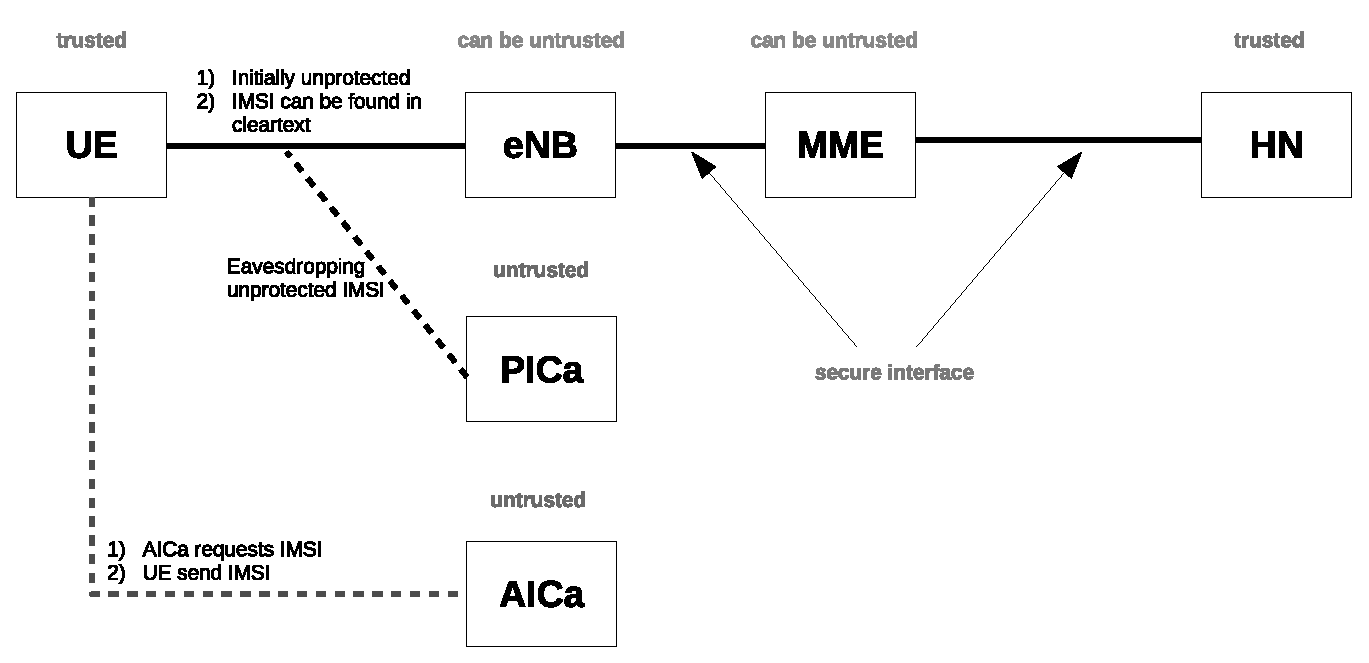
\includegraphics[height= 5cm]{security_architecture_abstraction.eps}
% figure caption is below the figure
\caption{High-level security architecture}
\label{fig:security_architecture_abstraction}       % Give a unique label
\end{center}
\end{figure} One approach of protecting IMSI privacy is to use a temporary identifier instead of the actual IMSI and keep changing the temporary identifier at a feasible frequency. Note that the temporary identifier has to be assigned over a confidentiality protected channel and different entities of the network may assign different temporary identifiers to the UE. In the LTE network, the temporary identifier assigned by a serving network (SN) is called globally unique temporary identity (GUTI) and the home network (HN) does not assign any temporary identifier to the UE. However, during the initial attachment of a UE to the SN, the UE has neither a GUTI nor a security context with the SN that can assign it with a GUTI. Besides, GUTI can be lost by either one or both of the UE and the SN. This would force the UE to reveal its IMSI to the SN to keep itself from permanently locked out of the network. This problem gives an opportunity to an AIC who impersonates a legitimate SN and forces the UE to run the initial attachment protocol. This also gives an opportunity to a PIC to eavesdrop the IMSI sent in clear text. Solutions \cite{pseudonym_valtteri_philip, pseudonym_ericsson} have been proposed by using temporary IMSI known as pseudonym assigned by the HN. While these solutions solve the cases of lost and unsynchronised GUTI, they still have the problem of lost or unsynchronised pseudonyms and also initial attachment. Public-key technologies have also been considered as potential approach to solve this problem

%In this report we present how a security context can be set up in between the network (either SN or HN) and the UE even before the identification of the UE so that the UE can use the security context to send its IMSI with confidentiality protection. Such a security context will mitigate the attack mounted by a PIC. In addition to this, we show that an AIC would not be able to agree on a legitimate security context with the UE and consequently will not be able to find out the IMSI.

In this paper we discuss different solutions based on pseudonyms and public-key encryption from a high level. The pseudonym based approaches require to maintain a synchronization of pseudonyms in between the UE and the HN. It is also difficult to resynchronize the pseudonyms once the synchronization is lost. We discuss solutions based on certificate based public-key and also root-key based pubic-key. Unlike the pseudonym based solutions these public-key based solutions do not require any synchronization. Then, we also propose a solution based on identity based encryption (IBE) that prevents both PIC and AIC. One additional benefit of our solution is, it also works as a mutual authentication protocol in between SN and UE without the involvement of the HN every time the authentication runs. This additional benefit is impossible to achieve using root-key based approach. Even though the aforementioned additional benefit is possible to achieve using certificate based approach, the certificate based approach has other downsides. 

Apart from preventing AIC and PIC, there are other 5G requirements which a solution should also meet. Reduced signalling overhead, improved control plane latency are two such requirements. Concealing all the parts of IMSI, namely, MCC, MNC and MSIN has been identified as another requirement. Also, in the case of public-key, the complexity involved in setting a PKI and revocation of a public-key need to be considered with high importance. In some cases the public key of an entity is pre-provisioned to all the potential senders in the system. If this public key is revoked and a new public-private key pair is generated by the entity from which the public key was revoked, then the new public key needs to be re-provisioned to all those entities that were pre-provisioned with the old public key. Considering all these requirements, we evaluate our solutions based on the following criteria: (1) Concealed from PIC, AIC, SN (2) Parts of the IMSI concealed (3 ) Signalling overhead (4) Latency (5) PKI complexity (6) Public-key revocation and re-provisioning 
\textcolor{red}{This list needs to be modified further.} %We also want to see if any of these solutions would work in a heterogeneous situation where one or more of the entities involved would come from the legacy networks. Apparently, none of the legacy networks use public-key encryption. Consequently, all of the solutions that use public-key encryption will not work in such a heterogeneous situation. A variant of pseudonym based approach might be possible to devise that work in some heterogeneous situation. 
While the choice of the solution is dependent on how much we want to achieve, our solution based on IBE becomes a competitive one by meeting most of the important requirements.

%In Section \ref{sec:id_based_crypto} we present a quick introduction to the different kinds of public-key encryption we have used in this report. 
In Section \ref{sec:existing_solutions} we present high-level discussions of different published solutions based on pseudonyms and different kinds of public-key encryption. In section  \ref{sec:solutions_based_on_IBE}, we present a solution based on IBE that is not only identification but also works as mutual authentication. In Section \ref{sec:evaluation}, we present an evaluation of the discussed presented solution along with our proposed solution based on the aforementioned evaluation criteria. Finally we conclude the paper in Section \ref{sec:conclusion}.




\section{Discussion on Different Solutions}\label{sec:solutions} 
\label{sec:existing_solutions}
It is beneficial to introduce some notation here before delving into the solutions. 
\begin{enumerate}
\item $hnid=MCC||MNC$ identifies the HN
\item $snid=MCC||MNC$ identifies the SN
\item $e_A$ is the public key of entity $A$
\item $d_A$ is the private key of entity $A$ 
\item $\mathcal{X}_{A,B}(e_A,e_B)$ is the certificate of the public key $e_A$ of $A$. The certificate can be verified by anyone who considers $B$ as a root CA using the public key $e_B$. The certificate is a guarantee from B that the public key $e_A$ is owned by $A$ .
\item $E,D$ are the encryption and decryption functions so that $D(E(M,K),K) = M$.
\item $S(M,K)$ is the signature of message $M$ signed by the key $K$
\end{enumerate}

\subsection{Solution Based on Pseudonyms:}
\label{sec:pseudonyms}


\subsection{Solution Based on Certificate Based Public-key Encryption} 
\label{sub_sec:solution_certificate}
To use certificate based public-key cryptography to secure IMSI privacy, we need to figure out a few things first: who are the root CAs and who else can be a CA, who are the entities that own a public key, how a certificate can be revoked, and how the UE can be re-provisioned with a new root certificate if required. Different solutions can be devised based on the choice of root CAs and other CAs. All those solutions will require an SN to have a valid certificate that a UE can verify using a public-key that the UE trusts. Consequently the root public-key has to be provisioned to all the UE. An SN has to obtain a certificate verifiable by all the UE the SN intends to serve. 

For an example, we can choose the HN of a subscriber as the root CA for the subscriber. In this case, the HN generates a public-private key pair and generates a certificate of the public key signed by the HN itself. A UE is provisioned with this self signed certificate. An SN interested to serve a UE obtains a certificate from the UE's HN. SN sends its public key $e_{snid}$ and $snid$ to the HN. The HN generates a certificate $\mathcal{X}_{snid,hnid} (e_{snid},e_{hnid})$. When the SN broadcasts its identity, the UE sends $hnid,e_{hnid}$ to the SN. The SN looks up for the certificate $\mathcal{X}_{snid,hnid} (e_{snid},e_{hnid})$. In case it exists at the disposal of the SN, the SN sends $\mathcal{X}_{snid,hnid} (e_{snid},e_{hnid})$ to the UE. The UE verifies the certificate and extracts the public key $e_{snid}$ from the certificate. If the certificate is verified as valid, then the UE sends the IMSI to the SN encrypted by the public key of the SN $e_{snid}$.  Note that the SN does not need to get the certificate from the HN, but the SN can get it from any CA who is trusted in by the HN in the chain of trust.


\subsection{Solution Based on Pre-provisioned Public Kyes of SNs} 
\label{sub_sec:solution_certificate_short_chain_pre-provisioned_keys}
The UE is periodically provisioned by the HN with the public key of the probable SNs the UE might visit in near future. If the SN asks for the IMSI from the UE, the UE looks for a public key of the SN in the key-table of the UE provisioned by HN. If it finds a matching public key $e_{snid}$, it encrypts the IMSI with the public key and sends the ciphertext to the SN along with $e_{snid}$ without asking a certificate for the public key from the SN.



\subsection{Solution based on Root-key based Encryption} 
\label{sub_sec:solution_root-key}
In root-key based public-key encryption, there is only a very limited number of public-private key pairs in the network. All the senders in the network are pre-provisioned with the public key of the receivers. We use only one pair of public-private key pair in this approach. This key pair is owned by the HN and we call it to be the root-key. The public key is provisioned to all the UE by the HN which have subscriptions with the HN. Whenever a UE is in need of identifying itself to an SN with the IMSI, the UE encrypts the IMSI with the public root key and sends the result to the SN along with the $hnid$. The SN sends the encrypted IMSI to the appropriate HN. HN decrypts and extract the IMSI. HN sends back the IMSI to the SN along with an authentication vector (AV) for running an authentication protocol in between the UE and the SN.


In the next section we discuss the basic principles of IBE and present a solution of the identity privacy using IBE. The solution is extended to a mutual authentication and key agreement protocol.


\section{Solution based on IBE} 
\label{sec:solutions_based_on_IBE}
In IBE the public and private key of a receiver is computed from the identity of the receiver in conjunction with the public and private key of a trusted third party respectively. As the private key of the trusted third party is required to compute the private key of the receiver, the private key of the receiver has to be provisioned to the receiver by the trusted third party. Even though an extra one-time burden of private key provisioning is required, a sender does not need to authenticate the public key of a receiver each time the sender and the receiver agree on a security context. The sender does not need to authenticate the public-key, because if the public key is not authentic, the receiver will not have the private key. If the receiver does not have the private key, any message encrypted by the public key will never be decrypted by the receiver. On the other hand the private key of the receiver would be provisioned to the receiver only if the receiver can authenticate itself to the trusted third party. In other words, the authenticity of the public key in IBE is guaranteed by the trusted third party. Usually in IBE, the trusted third party is known as the private key generator (PKG). While in the certificate based and root-key based cases it is possible to revoke the public key of a receiver, it is impossible to revoke the public key in IBE unless the identity itself is revoked. Please note that, a PKG knows the private keys of all the receivers whose public keys were generated using the PKG's public key. As a result a PKG can decrypt any message sent by any sender to any receiver. This assumes a very high level of trust in the PKG.  

RFC 6508 \cite{RFC6508} presents an algorithm called SAKKE for establishment of a secret shared value. Applications of SAKKE may include a date-time component in their identifier format to ensure that identifiers and hence the corresponding private-keys are only valid for a fixed period of time. 
Solution \#7.11 in 3GPP TR 33.899 \cite{TR33899} uses IBE to protect the long-term identifier according to RFC 6508. However, the solution doesn't address the issue of revocation of the identity based public-keys. RFC 6507 \cite{RFC6507} describes a certificate less signature scheme based on IBE. In this scheme a string called public validation token (PVT) randomly chosen by the PKG is assigned to an identity. Both the public and private key of an identity is computed using the PVT along with the identity. So, the public key associated with an identity can be revoked by revoking the PVT. Solution \#2.14 in 3GPP TR 33.899 presents an authentication framework based on the signature scheme of RFC 6507 and the authentication protocol EAP-TLS. This solution uses the PVT to revoke the public key associated with an identity.

Here we present a unified protocol that serves the purpose of privacy protected identification of UE and mutual authentication in between UE and SN. This mutual authentication does not require to contact with the HN each time it runs in between a UE and an SN. In our solution we do not use PVT but use an agreed expiry time. One candidate for such expiry time could be for example, the end of the current day. This expiry time can act as the PVT. If the public key of an identifier needs to be revoked, the expiry time along with the identifier is added to the revocation list. If the identity requires a new public key, the PKG uses another expiry time to compute the private key of the identity. The newly computed private key is then provisioned to the identity along with the the new expiry time. When the expiry time comes, all the public keys computed using the expiry time is automatically revoked. So, the revocation list does not need to maintain the history of revocation after the expiry time.


\begin{figure}
\begin{center}
% Use the relevant command to insert your figure file.
% For example, with the graphicx package use
  \includegraphics[height=9cm]{solution_based_on_ibc.eps}
% figure caption is below the figure
\caption{Privacy protected UE identification and mutual authentication using IBE}
\label{fig:solution_ibc}       % Give a unique label
\end{center}
\end{figure}

\subsubsection{Description of the solution}
The UE's HN acts as the PKG. The solution is pictorially presented in Figure \ref{fig:solution_ibc}. It has two different phases. In the first phase, the HN generates a public-private key pair $e_{hnid},d_{hnid}$ in step $1.1$. In step $1.2$, the HN provisions the UE with the public key $e_{hnid}$ and the private key $d_{ue}$. The private key $d_{ue}$ is generated using the private key $d_{hnid}$, a chosen expiry time $ET_{eu}$. The SN sends the $snid$ to HN in step $1.3$. In step $1.4$ the HN chooses a suitable expiry time $ET$ to generate the private key of the SN. The expiry time is appended with $snid$ and the private key $d_{snid}$ is computed considering $snid||ET$ as the identity of the SN. In step $1.5$, the HN sends $d_{snid}$ to the SN along with $ET$ and $e_{hnid}$. The SN stores these information in its key-table. The second phase is the identification phase. In step $2.1$, the SN broadcasts the $snid$. In step $2.2$ the UE sends $hnid,E(IMSI||ET_{ue}||RAND1,e_{snid}),ET$ to the SN. In step $2.3$ the SN looks for an appropriate private key $d_{snid}$ compatible with $ET$. If SN has such a private key then it jumps to step $8$. Otherwise it continues from step $2.4$ and stop at step $2.7$. In step $2.4$ SN sends $snid,E(IMSI||ET_{ue}||RAND1),ET$ to HN. In step $2.5$ HN computes the key $d_{snid}$ using $d_{hnid},snid$ and $ET$. Then HN decrypts the received encrypted message using the key $d_{snid}$. After extracting the the IMSI from the decrypted message, HN prepares an $AV$ that can be used in EPS-AKA. In step $2.6$, HN sends the $AV$ along with the $IMSI$ and $d_{snid}$. In step $2.7$ EPS-AKA is run in between UE and SN and consequently mutual authentication and key agreement is achieved.

However, if SN finds an appropriate $d_{snid}$ in step $2.3$, then the protocol jumps to step $2.8$. In step $2.8$ SN decrypts the received encrypted message and compute $e_{eu}$ using $IMSI||ET_{eu}$ and $e_{hnid}$. In step $2.9$ HN sends the signature $S(IMSI||RAND1||RAND2,d_{snid})$ along with $E(RAND2,e_{ue})$ to the UE. The signature is verifiable by $e_{snid}$. In step $2.10$ the UE sends the signature $S(IMSI||RAND1||RAND2,d_{ue})$ to the SN which is verifiable by $e_{ue}$. If both UE and SN can verify the signatures as valid, the mutual authentication is completed successfully.

Note that UE and SN have successfully exchanged two randomly chosen values RAND1 and RAND2 with confidentiality protection. A symmetric key can be computed at both UE and SN using these random values and $e_{hnid}$ in a function like $f3$ or $f4$ used in LTE security. There is also an alternative option of using ephemeral diffie-hellman key exchange protocol. The messages required for the ephemeral diffie-hellman key exchange can be transported along with the messages sent in step $2.9$ and $2.10$. In that case, confidentiality protection of $RAND2$ is not required.

\subsubsection{Revocation of Public Keys SNs}
As the public key in IBE can not be revoked, we use the concept of expiry time as the part of the identity of an entity. The expiry time is a time stamp in the future and acts as a PVT. So, when a public key needs to be revoked, the corresponding identifier and expiry time is put in a revocation list. Any sender encrypting a message using a public key should first check in the revocation list if the relevant identifier and expiry time is revoked or not. But for a UE it is not possible to access the revocation list because it does not yet have a security context with the SN. To circumvent this problem, HN gives the private key $d_{snid}$ to an SN for a short period of time, for an example, the day end. So, if the public key needs to be revoked, it would automatically be revoked when the expiration time comes. In this way, a compromised SN would be able mount an attack only for a short period of time. However, the SN would need to get new $d_{snid}$ from the HN before the expiry time of old $d_{snid}$ expires. On the other hand, when the public key of a UE is revoked, the IMSI and relevant expiry time is stored in a revocation list in the HN.  An SN serving UEs of an HN has a copy of the list. The SN also periodically checks with the HN if there is any new revocation. Before computing the public key of the UE in step $2.8$, the SN checks the revocation list if the $IMSI||ET_{ue}$ is revoked or not. If it is revoked, the SN discards the message received from the UE and authentication fails. As revocation of the public key of a UE is possible to be checked in a revocation list, UEs can be given private keys associated with expiry time which is fairly ahead in future, e.g., for a year. And all the entries with expiry time older than current date-time be removed from the revocation list, hence the revocation list will not grow to an extreme size. This frequent private key exchange and refreshing the revocation list would create a bit increased traffic in between an SN and HN. On the other hand, this increased traffic is not in the air interface but in the back haul network, which apparently is not very critical. 


\section{Evaluation}
\label{sec:evaluation}
We have discussed the the pros and cons of different solutions in their respective subsections in Section \ref{sec:solutions}. All the solutions conceal the MSIN from both AIC and PIC and reveals the entire IMSI to SN. That is why we do not mention the concealment of IMSI as a comparing criterion.  Table \ref{table:comparison} shows a quick comparison. Note that this is a local comparison, not a global one. For an example, when we say the signalling overhead is low, we mean that it is low comparing with other solutions presented in this report. 
\begin{table}
\begin{center}
\begin{tabular}{ |p{3.5cm}|p{2cm}|p{2cm}|p{2cm}|p{2cm}|  }
\hline
\textbf{Solutions} & \textbf{Signalling Overhead} & \textbf{Latency} & \textbf{PKI Effort} & \textbf{Key revocation and re-provisioning}\\
\hline \hline
Pseudonym based & ?? & ?? & ?? & ?? \\ \hline
Certificate based & high & high & high & possible and complex\\ \hline
Based on pre-provisioned public keys of SNs & low & low & low & possible and easy \\ \hline
Root-key based & low & low & low & possible and easy \\ \hline
IBE based & low & low & low & possible and easy \\ \hline
\end{tabular}
\vspace{5pt}
\caption{Comparative evaluation of the solutions}
\label{table:comparison}
\end{center}
\end{table}


%\begin{figure}
%\begin{center}
% Use the relevant command to insert your figure file.
% For example, with the graphicx package use
%  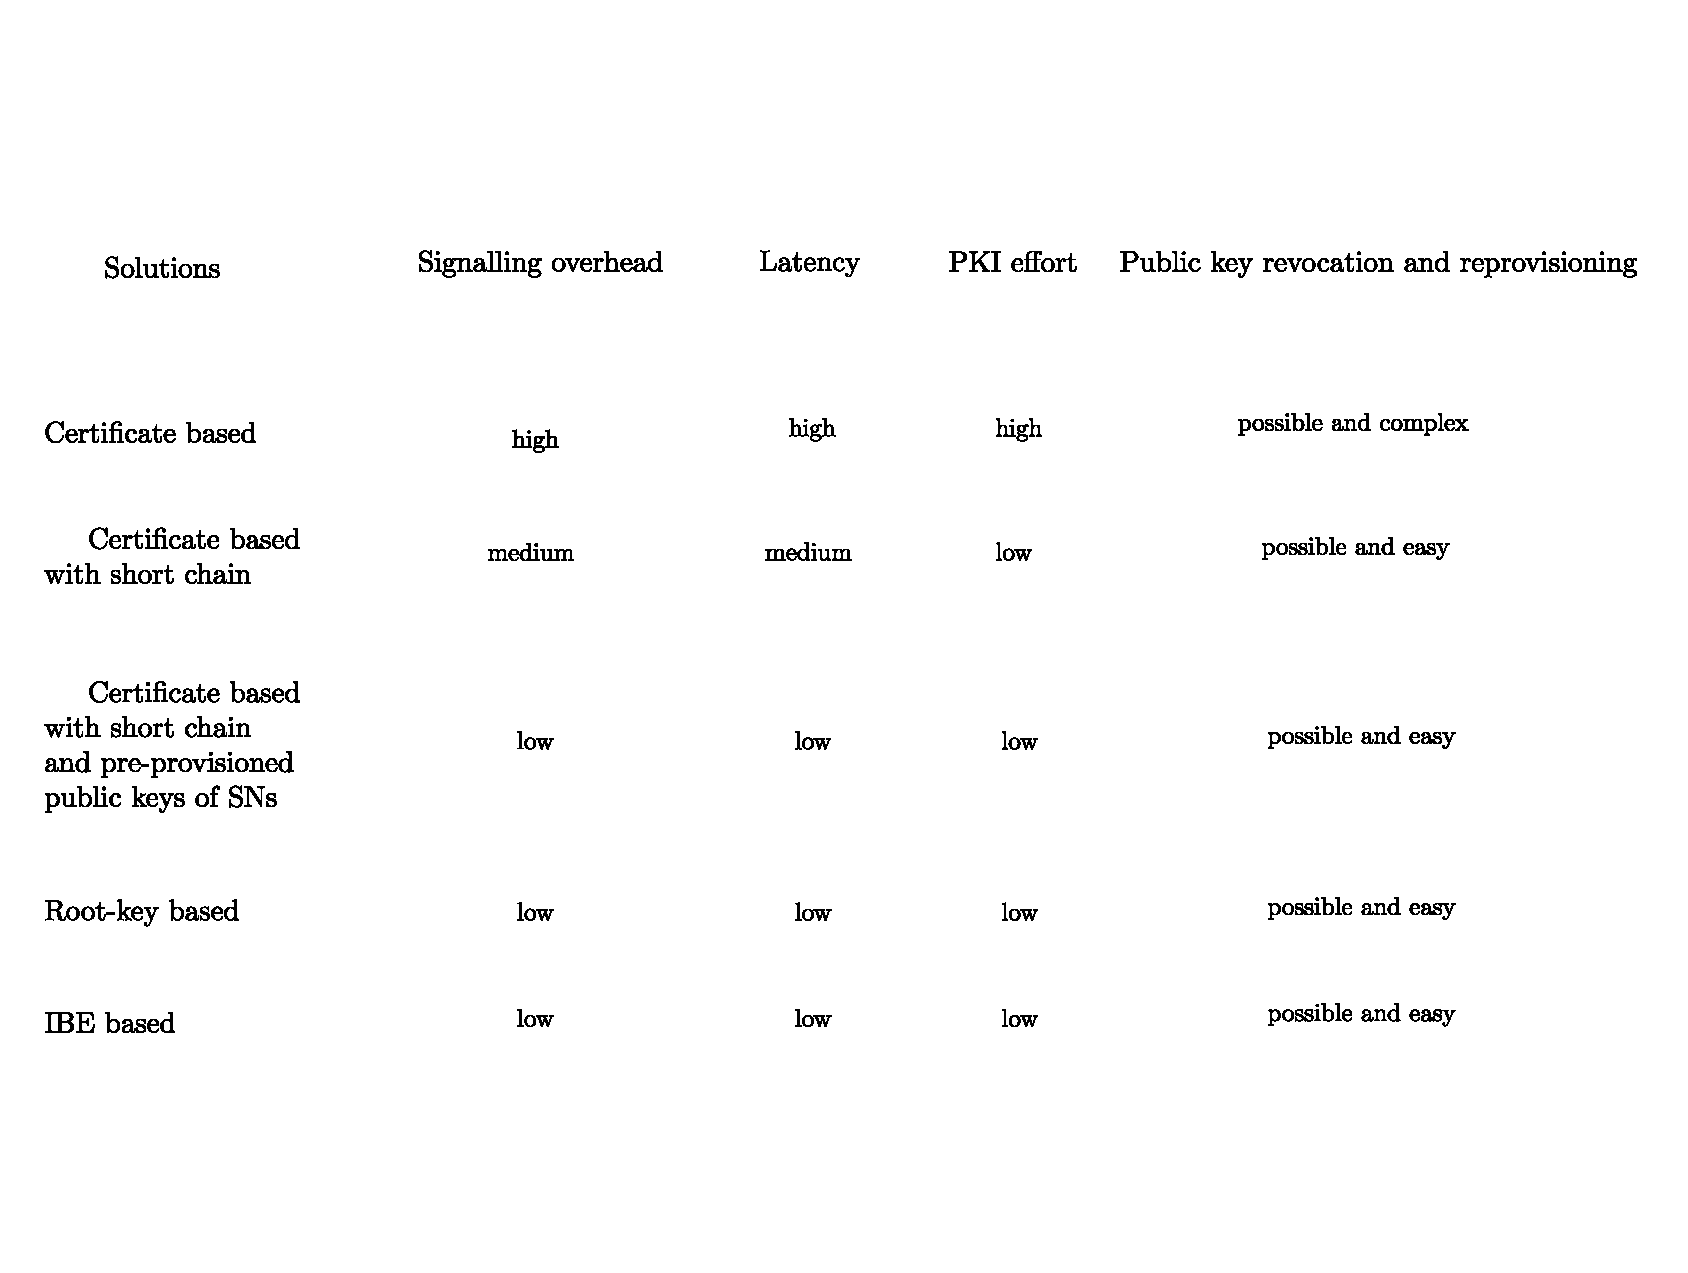
\includegraphics[width=.98\textwidth]{compare.eps}
% figure caption is below the figure
%\newline
%\caption{Comparison among the solutions}
%\label{fig:solution_ibc}       % Give a unique label
%\end{center}
%\end{figure}

All the solutions are based on public-key encryption. As a result all of them requires expensive computation of public-key encryption. Another downside of public-key encryption is the size of the ciphertext is comparatively large. These two downsides will affect the latency and signalling overhead. Once a UE is identified and authenticated by the SN, the SN assigns a GUTI to the UE. In the consecutive identification and authentication, this GUTI can be used. However, when the GUTI is not synchronised in between the SN and the UE, or the UE tries to connect to a new SN, the GUTI does not work. In that situation, the solutions we have proposed can be used. Hence, solutions of public-key encryption based solution is not required to run each time there is a need of identification of a UE. By using a temporary identifier assigned to the UE by the HN, we can reduce the need of running the public-key encryption based solution. The temporary identifier assigned by the HN is called pseudonym. Solutions based on pseudonyms have been proposed in \cite{pseudonym_valtteri_philip,pseudonym_ericsson}. By using the public-key encryption based solution in conjunction with GUTI and pseudonym, the need for running the public-key encryption based solution becomes very infrequent. Besides, the need of low latency is mostly for making the tactile internet successful. As a result, it is the data plane where the low latency is critical, not the control plane. However, it is still a matter of further research to quantify the impact of public-key encryption on signalling overhead and latency. 



\section{Conclusion}
\label{sec:conclusion}
In this report we have discussed different solutions based on public-key encryption to protect the privacy of the long-term identifier known as IMSI. We have come up with a categorisation of public-key encryption and presented one solution using each of the subcategories. The comparative analysis among the techniques from different categories of public-key encryption shows that pre-provisioned public keys of the SNs, root-key and IBE based solutions are promising approaches to protect the IMSI privacy.
Interestingly, none of the solutions need a new entity to build the PKI. However, as all the solutions are based on public-key encryption, the expensive computation and longer ciphertext are the inherent downsides of all the solutions. These downsides affect the latency and signalling overhead. In conjunction with GUTI and pseudonym the impact on latency and signalling overhead can be reduced to large extent. However, quantification of the latency and signalling overhead remains open to further research.


\begin{thebibliography}{4}

\bibitem{NGMN_white_paper} NGMN 5G White Paper V1.0 [cited Jan, 2017]. Available at: https://www.ngmn.org/uploads/media/\\NGMN\_5G\_White\_Paper\_V1\_0.pdf

\bibitem{TR33899} 3GPP TR 33.899 V0.6.0 [cited Jan, 2017]. Available at: https://portal.3gpp.org/desktopmodules/Specifications/\\SpecificationDetails.aspx?specificationId=3045

\bibitem{TS23003} 3GPP TS 23.003 V14.2.0 [cited Jan, 2017]. Available at: https://portal.3gpp.org/desktopmodules/Specifications/\\SpecificationDetails.aspx?specificationId=729

\bibitem{TR21905} 3GPP TR 21.905 [cited Jan, 2017]. Available at: https://portal.3gpp.org/desktopmodules/Specifications/\\SpecificationDetails.aspx?specificationId=558


\bibitem{pseudonym_ericsson} Karl Norrman, Mats N\"aslund, Elena Dubrova: Protecting IMSI and User Privacy in 5G Networks. 2nd International Workshop on 5G Security

\bibitem{pseudonym_valtteri_philip} Philip Ginzboorg,  Valtteri Niemi: Privacy of the long-term identities in cellular networks. Proceedings of the 9th EAI International Conference on Mobile Multimedia Communications
Pages 167-175

\bibitem{RFC6507} 3GPP TR 21.905 [cited Jan, 2017]. Available at: https://portal.3gpp.org/desktopmodules/Specifications/\\SpecificationDetails.aspx?specificationId=558

\bibitem{RFC6508} 3GPP TR 21.905 [cited Jan, 2017]. Available at: https://portal.3gpp.org/desktopmodules/Specifications/\\SpecificationDetails.aspx?specificationId=558

\bibitem{TS33106} 3GPP TS 23.003 V14.2.0 [cited Jan, 2017]. Available at: https://portal.3gpp.org/desktopmodules/Specifications/\\SpecificationDetails.aspx?specificationId=729

\bibitem{TS33107} 3GPP TS 23.003 V14.2.0 [cited Jan, 2017]. Available at: https://portal.3gpp.org/desktopmodules/Specifications/\\SpecificationDetails.aspx?specificationId=729


\end{thebibliography}

\end{document}
